\chapter{Recreating winning approach}\label{sec:recreating}
In this chapter, the classification method of the Ford Competition winner will be attempted to be recreated. The goal is to get a result -- as measured by the AUC -- that is close to the winners approach.

\section{The winning approach}
The competition winner has described his approach in \citet{inference_winning_approach}, which will just be called ``the paper'' in the rest of this section. \par
In the paper two key observations are mentioned. First of all, the winner observed that in most of the trials, the driver was either alert most of the time, or not alert for most of the time. Secondly the winner observed that there was a mismatch between the AUC-scores achieved on the trainingset and on the testset. Since it wasn't possible to get access to the testset of the competition, the second observation isn't of any direct use for this report. The two observations though, gives an explanation of why the winner chose the model he did. \par
Since most trials was either alert-trials or not-alert-trials, the winner thought it would make sense to calculate aggregated features within trials. He therefore included the mean and the standard deviation of all features, aggregated backwards, within a trial. As a standard the mean features was prefixed ``m'' and the standard deviation ``sd''. 
\begin{Exa}
    In the $k$'th observation of trial $t$, the value of feature \fn{mP6}, is the mean of feature \fn{P6}, for observation $0,1,2,\dots,k-1$ in trial $t$
\end{Exa}
The fact that there was a mismatch between the trainingset and testset of the competition, made the winner focus on simple models, since he expected that the trainingset wasn't capturing all aspects of the testset, and extrapolation was therefore needed.

\subsection{Classification method}
The method used by the winner was a logistic regression, trained on the three features \fn{sdE5}, \fn{V11} and \fn{E9}. The three features was selected ``... based on diagnostics of the logistic regression ...'' \citep[p.3]{inference_winning_approach}. The final model was a logistic regression with the following weights
\[
    \log\frac{P(t=0|\ve{x})}{P(t=1|\ve{x})} = -392.4317\cdot\text{sdE5} + 0.2209\cdot\text{V11} + 3.6544\cdot\text{E9}
\]
\begin{figure}
    \centering
    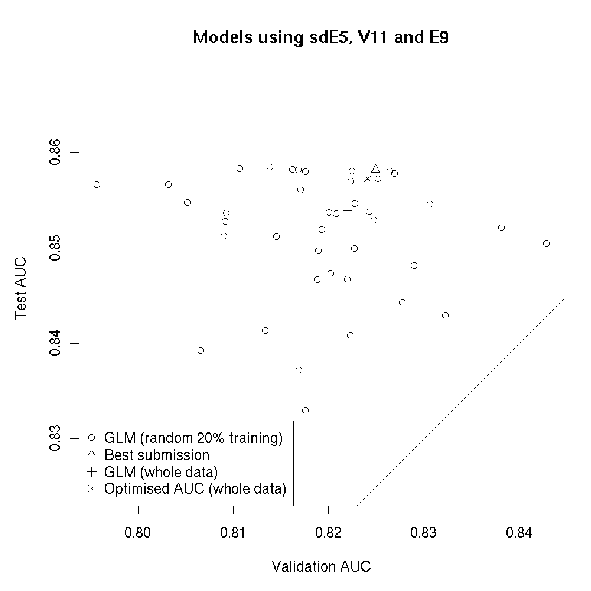
\includegraphics[width=100mm]{media/fig2-inference-paper.pdf}
    \caption{Reproduction of figure 2 in \citet{inference_winning_approach}. The models that achieves a Test AUC higher than 0.8492 are using future observations to predict the \fn{IsAlert} feature, which wasn't allowed in the competition. See \citet{inference_winning_approach} for more information.}\label{fig:auc-score-inference-paper}
\end{figure}
The winner do not mention any intercept parameter, although it seems unlikely that no intercept was included in the model \citep{meetings-morten}. Based on the above parameters, the winner achieved an AUC-score of 0.8492 on the testset. As mentioned in the previous section, the AUC-score of the testset differed from the AUC-score on the trainingset. In figure~\ref{fig:auc-score-inference-paper} (a reproduction of a figure in \citet{inference_winning_approach}) it is seen that an AUC-score of 0.8492 on the testset, corresponded to a AUC-score of $0.82\pm0.01$ on the trainingset. Since only the trainingset is available for this report, the goal is to acieve an AUC-score of approximately $0.82\pm0.01$.

\section{Recreating the winning approach}
It is now time to recreate the logistic regression of the winner. Using the same features as the winner a logistic regression is trained on the trainingset. This resulted in the following model 
\begin{equation}\label{eq:winner-recreated}
    \log\frac{P(t=0|\ve{x})}{P(t=1|\ve{x})} = -87.2753\cdot\text{sdE5} + 0.2244\cdot\text{V11} + 3.6545\cdot\text{E9} - 5.3645 
\end{equation}
The model is much like the winning model. The highest deviation from the winning model is in the weight of feature \fn{sdE5}. To make it possible to calculate a confidence interval for the AUC-score of the new model, the testset is split in 10 parts, and an AUC-score is calculated for each part. The results can be seen in table~\ref{tbl:recreate-results} and the source code used to calculate the results can be found in \appref{source-recreate-winner} \par
\begin{table}
    \centering
    {\sffamily\small
        \begin{tabularx}{30mm}{ l R }
        Run & AUC \\\hline
        1 & 0.8082 \\
        2 & 0.8050 \\
        3 & 0.8114 \\
        4 & 0.8088 \\
        5 & 0.8063 \\
        6 & 0.8020 \\
        7 & 0.8128 \\
        8 & 0.8116 \\
        9 & 0.8057 \\
        10 & 0.8104 \\
        \end{tabularx}
    }
    \caption{Results of calculating the AUC-score for the model in equation~\eqref{eq:winner-recreated}, for 10 parts of the testset.}
    \label{tbl:recreate-results}
\end{table}
From the results table it is seen that the AUC-score achieved by the model lays in the interval [0.805;0.813] which is very close to the goal of $0.82\pm0.1$. To get a better idea of the results of the model, summary statistics and a confidence interval are calculated.

\subsection{Statistics on the AUC score}
As described in section~\ref{sec:statistics-on-performance} a 95\% confidence interval can be calculated from the sample mean and standard deviation. These are found as
\[
    m = 0.8082 \quad\quad\text{and}\quad\quad s = 0.003456
\]
which gives the confidence interval
\begin{align*}
    95\%\:\text{CI} &= [0.8082-2.2622\frac{0.003456}{\sqrt{10}}, 0.8082+2.2622\frac{0.003456}{\sqrt{10}}]\\
    &= [0.8058, 0.8107]
\end{align*}
that should be interpreted as 
\[
    \CI{0.8058}{0.8107}
\]
